% This file was created by tikzplotlib v0.9.1.
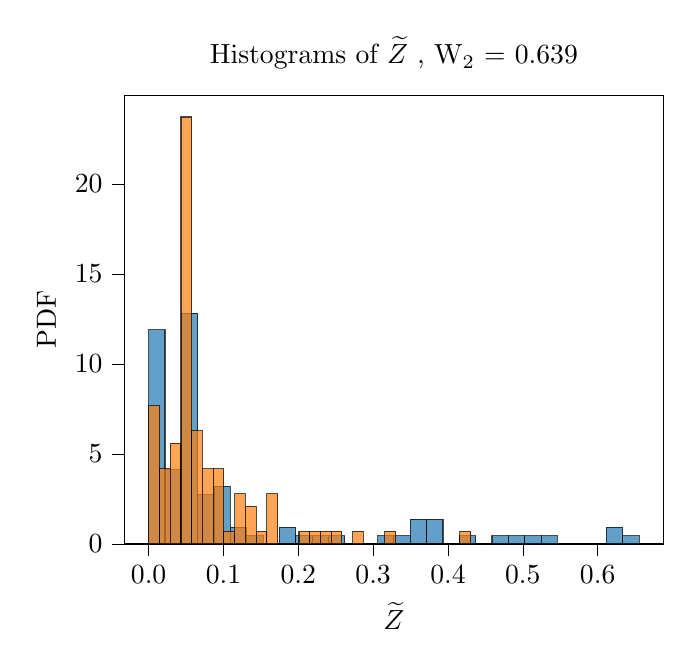
\begin{tikzpicture}

\definecolor{color0}{rgb}{0.12156862745098,0.466666666666667,0.705882352941177}
\definecolor{color1}{rgb}{1,0.498039215686275,0.0549019607843137}

\begin{axis}[
legend cell align={left},
legend style={fill opacity=0.8, draw opacity=1, text opacity=1, draw=white!80!black},
tick align=outside,
tick pos=left,
title={Histograms of \(\displaystyle \widetilde{Z}\) , W\(\displaystyle _2\) = 0.639},
x grid style={white!69.0196078431373!black},
xlabel={\(\displaystyle \widetilde{Z}\)},
xmin=-0.0327745998848679, xmax=0.688266596999587,
xtick style={color=black},
xtick={-0.1,0,0.1,0.2,0.3,0.4,0.5,0.6,0.7},
xticklabels={\(\displaystyle -0.1\),\(\displaystyle 0.0\),\(\displaystyle 0.1\),\(\displaystyle 0.2\),\(\displaystyle 0.3\),\(\displaystyle 0.4\),\(\displaystyle 0.5\),\(\displaystyle 0.6\),\(\displaystyle 0.7\)},
y grid style={white!69.0196078431373!black},
ylabel={PDF},
ymin=0, ymax=24.9120978024676,
ytick style={color=black},
ytick={0,5,10,15,20,25},
yticklabels={\(\displaystyle 0\),\(\displaystyle 5\),\(\displaystyle 10\),\(\displaystyle 15\),\(\displaystyle 20\),\(\displaystyle 25\)}
]
\draw[draw=black,fill=color0,opacity=0.7] (axis cs:-2.64836139129976e-11,0) rectangle (axis cs:0.0218497332124393,11.8994587786014);
\draw[draw=black,fill=color0,opacity=0.7] (axis cs:0.0218497332124393,0) rectangle (axis cs:0.0436994664513621,4.11904342336203);
\draw[draw=black,fill=color0,opacity=0.7] (axis cs:0.0436994664513621,0) rectangle (axis cs:0.065549199690285,12.8148017615708);
\draw[draw=black,fill=color0,opacity=0.7] (axis cs:0.065549199690285,0) rectangle (axis cs:0.0873989329292079,2.74602894890802);
\draw[draw=black,fill=color0,opacity=0.7] (axis cs:0.0873989329292079,0) rectangle (axis cs:0.109248666168131,3.20370044039269);
\draw[draw=black,fill=color0,opacity=0.7] (axis cs:0.109248666168131,0) rectangle (axis cs:0.131098399407054,0.915342982969341);
\draw[draw=black,fill=color0,opacity=0.7] (axis cs:0.131098399407054,0) rectangle (axis cs:0.152948132645976,0.45767149148467);
\draw[draw=black,fill=color0,opacity=0.7] (axis cs:0.152948132645977,0) rectangle (axis cs:0.174797865884899,0);
\draw[draw=black,fill=color0,opacity=0.7] (axis cs:0.174797865884899,0) rectangle (axis cs:0.196647599123822,0.91534298296934);
\draw[draw=black,fill=color0,opacity=0.7] (axis cs:0.196647599123822,0) rectangle (axis cs:0.218497332362745,0.45767149148467);
\draw[draw=black,fill=color0,opacity=0.7] (axis cs:0.218497332362745,0) rectangle (axis cs:0.240347065601668,0.45767149148467);
\draw[draw=black,fill=color0,opacity=0.7] (axis cs:0.240347065601668,0) rectangle (axis cs:0.262196798840591,0.45767149148467);
\draw[draw=black,fill=color0,opacity=0.7] (axis cs:0.262196798840591,0) rectangle (axis cs:0.284046532079514,0);
\draw[draw=black,fill=color0,opacity=0.7] (axis cs:0.284046532079514,0) rectangle (axis cs:0.305896265318437,0);
\draw[draw=black,fill=color0,opacity=0.7] (axis cs:0.305896265318437,0) rectangle (axis cs:0.327745998557359,0.45767149148467);
\draw[draw=black,fill=color0,opacity=0.7] (axis cs:0.32774599855736,0) rectangle (axis cs:0.349595731796282,0.45767149148467);
\draw[draw=black,fill=color0,opacity=0.7] (axis cs:0.349595731796282,0) rectangle (axis cs:0.371445465035205,1.37301447445401);
\draw[draw=black,fill=color0,opacity=0.7] (axis cs:0.371445465035205,0) rectangle (axis cs:0.393295198274128,1.37301447445401);
\draw[draw=black,fill=color0,opacity=0.7] (axis cs:0.393295198274128,0) rectangle (axis cs:0.415144931513051,0);
\draw[draw=black,fill=color0,opacity=0.7] (axis cs:0.415144931513051,0) rectangle (axis cs:0.436994664751974,0.45767149148467);
\draw[draw=black,fill=color0,opacity=0.7] (axis cs:0.436994664751974,0) rectangle (axis cs:0.458844397990897,0);
\draw[draw=black,fill=color0,opacity=0.7] (axis cs:0.458844397990897,0) rectangle (axis cs:0.48069413122982,0.45767149148467);
\draw[draw=black,fill=color0,opacity=0.7] (axis cs:0.48069413122982,0) rectangle (axis cs:0.502543864468743,0.457671491484669);
\draw[draw=black,fill=color0,opacity=0.7] (axis cs:0.502543864468743,0) rectangle (axis cs:0.524393597707665,0.457671491484671);
\draw[draw=black,fill=color0,opacity=0.7] (axis cs:0.524393597707665,0) rectangle (axis cs:0.546243330946588,0.457671491484669);
\draw[draw=black,fill=color0,opacity=0.7] (axis cs:0.546243330946588,0) rectangle (axis cs:0.568093064185511,0);
\draw[draw=black,fill=color0,opacity=0.7] (axis cs:0.568093064185511,0) rectangle (axis cs:0.589942797424434,0);
\draw[draw=black,fill=color0,opacity=0.7] (axis cs:0.589942797424434,0) rectangle (axis cs:0.611792530663357,0);
\draw[draw=black,fill=color0,opacity=0.7] (axis cs:0.611792530663357,0) rectangle (axis cs:0.63364226390228,0.915342982969343);
\draw[draw=black,fill=color0,opacity=0.7] (axis cs:0.63364226390228,0) rectangle (axis cs:0.655491997141203,0.457671491484669);
\draw[draw=black,fill=color1,opacity=0.7] (axis cs:0.000352393,0) rectangle (axis cs:0.0146827799,7.67599652176872);
\draw[draw=black,fill=color1,opacity=0.7] (axis cs:0.0146827799,0) rectangle (axis cs:0.0290131668,4.18690719369203);
\draw[draw=black,fill=color1,opacity=0.7] (axis cs:0.0290131668,0) rectangle (axis cs:0.0433435537,5.5825429249227);
\draw[draw=black,fill=color1,opacity=0.7] (axis cs:0.0433435537,0) rectangle (axis cs:0.0576739406,23.7258074309215);
\draw[draw=black,fill=color1,opacity=0.7] (axis cs:0.0576739406,0) rectangle (axis cs:0.0720043275,6.28036079053804);
\draw[draw=black,fill=color1,opacity=0.7] (axis cs:0.0720043275,0) rectangle (axis cs:0.0863347144,4.18690719369203);
\draw[draw=black,fill=color1,opacity=0.7] (axis cs:0.0863347144,0) rectangle (axis cs:0.1006651013,4.18690719369203);
\draw[draw=black,fill=color1,opacity=0.7] (axis cs:0.1006651013,0) rectangle (axis cs:0.1149954882,0.697817865615338);
\draw[draw=black,fill=color1,opacity=0.7] (axis cs:0.1149954882,0) rectangle (axis cs:0.1293258751,2.79127146246135);
\draw[draw=black,fill=color1,opacity=0.7] (axis cs:0.1293258751,0) rectangle (axis cs:0.143656262,2.09345359684602);
\draw[draw=black,fill=color1,opacity=0.7] (axis cs:0.143656262,0) rectangle (axis cs:0.1579866489,0.697817865615337);
\draw[draw=black,fill=color1,opacity=0.7] (axis cs:0.1579866489,0) rectangle (axis cs:0.1723170358,2.79127146246135);
\draw[draw=black,fill=color1,opacity=0.7] (axis cs:0.1723170358,0) rectangle (axis cs:0.1866474227,0);
\draw[draw=black,fill=color1,opacity=0.7] (axis cs:0.1866474227,0) rectangle (axis cs:0.2009778096,0);
\draw[draw=black,fill=color1,opacity=0.7] (axis cs:0.2009778096,0) rectangle (axis cs:0.2153081965,0.697817865615338);
\draw[draw=black,fill=color1,opacity=0.7] (axis cs:0.2153081965,0) rectangle (axis cs:0.2296385834,0.697817865615338);
\draw[draw=black,fill=color1,opacity=0.7] (axis cs:0.2296385834,0) rectangle (axis cs:0.2439689703,0.697817865615338);
\draw[draw=black,fill=color1,opacity=0.7] (axis cs:0.2439689703,0) rectangle (axis cs:0.2582993572,0.697817865615338);
\draw[draw=black,fill=color1,opacity=0.7] (axis cs:0.2582993572,0) rectangle (axis cs:0.2726297441,0);
\draw[draw=black,fill=color1,opacity=0.7] (axis cs:0.2726297441,0) rectangle (axis cs:0.286960131,0.697817865615338);
\draw[draw=black,fill=color1,opacity=0.7] (axis cs:0.286960131,0) rectangle (axis cs:0.3012905179,0);
\draw[draw=black,fill=color1,opacity=0.7] (axis cs:0.3012905179,0) rectangle (axis cs:0.3156209048,0);
\draw[draw=black,fill=color1,opacity=0.7] (axis cs:0.3156209048,0) rectangle (axis cs:0.3299512917,0.697817865615338);
\draw[draw=black,fill=color1,opacity=0.7] (axis cs:0.3299512917,0) rectangle (axis cs:0.3442816786,0);
\draw[draw=black,fill=color1,opacity=0.7] (axis cs:0.3442816786,0) rectangle (axis cs:0.3586120655,0);
\draw[draw=black,fill=color1,opacity=0.7] (axis cs:0.3586120655,0) rectangle (axis cs:0.3729424524,0);
\draw[draw=black,fill=color1,opacity=0.7] (axis cs:0.3729424524,0) rectangle (axis cs:0.3872728393,0);
\draw[draw=black,fill=color1,opacity=0.7] (axis cs:0.3872728393,0) rectangle (axis cs:0.4016032262,0);
\draw[draw=black,fill=color1,opacity=0.7] (axis cs:0.4016032262,0) rectangle (axis cs:0.4159336131,0);
\draw[draw=black,fill=color1,opacity=0.7] (axis cs:0.4159336131,0) rectangle (axis cs:0.430264,0.697817865615338);
\end{axis}

\end{tikzpicture}
